\section{Module 4: Hệ Động lực Rời rạc (Discrete Dynamical Systems)}
\label{sec:m4}

\subsection{Cơ sở Lý thuyết Hệ Động lực Rời rạc}
Theo chương 5 giáo trình \textit{Dynamical Systems -- Modeling Techniques in Practice} (CO2011) \cite{slides_dynamics,giordano2013,elaydi2005}, sự tiến hóa theo thời gian rời rạc (từng tuần) của hệ thống được mô tả bằng phương trình sai phân (\textit{difference equation}):

\begin{theorybox}{Cơ sở Lý thuyết Hệ Sai phân và Ổn định (CO2011 Slides Ch.5)}
\begin{itemize}
    \item \textbf{Phương trình sai phân tuyến tính (\texttt{Thm. 5.1--5.3}):} Xét hệ vô hướng bậc nhất $a_{n+1} = r a_n + b$. Một điểm $c$ gọi là \textit{điểm cân bằng} (\textit{equilibrium / fixed point}, \texttt{Def. 5.1}) nếu $c = f(c)$. Khi $r \neq 1$, hệ có điểm cân bằng duy nhất $c = \frac{b}{1-r}$ (\texttt{Thm. 5.2}) và nghiệm tổng quát dạng đóng $a_k = d r^k + c$ với $d = a_0 - c$ (\texttt{Thm. 5.3}). Khi $r = 1$ và $b \neq 0$, hệ không có điểm cân bằng.
    \item \textbf{Hệ động lực vector và Tiêu chuẩn ổn định:} Với hệ tuyến tính nhiều biến $F_{n+1} = A F_n + u$ ($F_n \in \mathbb{R}^N$), ma trận Jacobi là $J = A$. Gọi bán kính phổ $\rho(A) = \max_k |\lambda_k(A)|$ là trị tuyệt đối lớn nhất của các trị riêng. Điểm cân bằng $F^* = (I - A)^{-1} u$ là: (i) \textit{ổn định tiệm cận toàn cục} nếu $\rho(A) < 1$; (ii) \textit{trung hòa} nếu $\rho(A) = 1$; (iii) \textit{không ổn định} nếu $\rho(A) > 1$.
    \item \textbf{Phân biệt với bộ tích lũy thô:} Hệ cộng dồn tải trọng $w_{n+1} = w_n + A_n x_n$ có ma trận Jacobi $J = I$ (trị riêng bằng $1$) nên không có điểm cân bằng hữu hạn khác tầm thường. Động lực thực sự nằm ở cơ chế tích lũy có suy giảm (\textit{retention/decay}).
\end{itemize}
\end{theorybox}

\subsection{Lựa chọn Hướng B và Hiệu chuẩn Tham số từ Dữ liệu Thực}
\label{sec:m4_calib}

Trong ba hướng của đề bài, nhóm lựa chọn \textbf{Hướng B (Vector Fatigue \& Fairness)} vì hai lý do: (1) Hướng B liên kết trực tiếp phân bố tải công bằng với độ phân tán cân bằng của vector mệt mỏi trên toàn đội ngũ $73$ người; (2) Hướng A đòi hỏi tự giả lập chính sách phản hồi vòng kín, còn Hướng C cần nhãn trạng thái \textit{available/busy/on-leave} vốn không quan sát được từ dữ liệu gốc.

\paragraph*{Trích xuất tải tuần và hiệu chuẩn từ \texttt{Baseline} (\texttt{workload.py}, \texttt{fatigue.py}):}
Toàn bộ khung lịch $27$ ngày (18/05--13/06/2026) được chia thành $4$ khối tuần liên tiếp có độ dài $d = [7, 7, 7, 6]$ ngày, với tổng số lượt coi thi tương ứng là $[15, 103, 339, 312]$ ($769$ lượt). Với khối $k$ dài $d_k$ ngày, suất coi thi quy chuẩn tuần của cán bộ $i$ là $L_{k,i} = \frac{7\, c_{k,i}}{d_k}$, và tải trung bình tuần toàn kỳ là $\ell_i = \frac{7 \sum_k c_{k,i}}{27}$, có trung bình toàn khoa $\mu = \frac{769 \times 7}{73 \times 27} = 2{,}731101$ ca/tuần.

Vì tập dữ liệu không đo lường sinh lý học, nhóm định nghĩa $F_{n} \in \mathbb{R}^{73}$ là \textbf{đại lượng đại diện mệt mỏi theo đơn vị tải tuần} (\textit{workload proxy}) dưới các giả định tường minh:
\begin{enumerate}
    \item \textbf{Hệ số lưu giữ $a$:} Hồi quy OLS gộp trễ bậc 1 $L_{k+1,i} = \text{intercept} + a L_{k,i} + \varepsilon_{k,i}$ trên $219$ cặp $(\text{người}, \text{khối liền kề})$ thu được $a = 0{,}270634$ (hệ số chặn $3{,}115617$, $\text{RMSE} = 2{,}529817$, $R^2 = 0{,}061930$). Mức $R^2$ thấp do nhu cầu thi dồn mạnh về hai tuần cuối ($339$ và $312$ lượt so với $15$ lượt tuần đầu), hạn chế khả năng dự báo ngoại suy nhưng giữ tính minh bạch thống kê.
    \item \textbf{Hệ số nghỉ ngơi $r = 0$ và chuẩn hóa $b = 1 - a$:} Do không có dữ liệu nghỉ phép thực, đặt $r = 0$. Hệ số $b$ được chuẩn hóa để điểm cân bằng tại mức tải trung bình $\mu$ bằng chính $\mu$: $\frac{b \mu}{1 - a} = \mu \Rightarrow b = 1 - a = 0{,}729366$.
    \item \textbf{Nội suy tuần cuối $6$ ngày:} Theo nửa nhóm mũ liên tục, khối dài $d$ ngày dùng $\alpha_d = a^{d/7}$ và $\beta_d = b\,\frac{1 - \alpha_d}{1 - a}$, nên khối cuối ($d=6$) phản ánh chính xác $6$ ngày tích lũy và suy giảm.
\end{enumerate}

\subsection{Điểm Cân bằng, Phân loại Ổn định và Liên kết với Công bằng}
\label{sec:m4_stability}

Xét hệ thức sai phân vector cho tải trung bình tuần hằng số $\ell \in \mathbb{R}^{73}$ và nghỉ $\rho \in \mathbb{R}^{73}$:
\begin{equation}
    F_{n+1} = a F_n + b \ell - r \rho, \qquad F^* = \frac{b\ell - r\rho}{1 - a} \;\; (a \neq 1), \qquad F_n = F^* + a^n (F_0 - F^*).
\end{equation}
Với hiệu chuẩn $r = 0$ và $b = 1 - a$, điểm cân bằng trùng khớp đúng vector tải tuần: $F^* = \ell$. Ma trận Jacobi của ánh xạ là $J = a I_{73}$, có toàn bộ $73$ trị riêng bằng $a = 0{,}270634$. Vì bán kính phổ $\rho(J) = |a| = 0{,}270634 < 1$, điểm cân bằng $F^*$ \textbf{ổn định tiệm cận toàn cục}. Bảng~\ref{tab:m4_regimes} đối chiếu kiểm chứng số sau $20$ tuần giữa các miền tham số:

\begin{table}[htbp]
\centering
\caption{Kiểm chứng phân loại ổn định của hệ động lực qua $20$ tuần mô phỏng.}
\label{tab:m4_regimes}
\small
\setlength{\tabcolsep}{5pt}
\renewcommand{\arraystretch}{1.22}
\begin{tabularx}{\textwidth}{@{} l L C C @{}}
\toprule
\textbf{Tham số $a$} & \textbf{Phân loại ổn định ($\rho(J)=|a|$)} & \textbf{Tỷ số khoảng cách lý thuyết $|a|^{20}$} & \textbf{Tỷ số đo trên mô phỏng} \\
\midrule
$a = 0{,}270634$ & \textbf{Ổn định tiệm cận toàn cục} & $4{,}4428 \times 10^{-12}$ & $4{,}4428 \times 10^{-12}$ \\
$a = 1{,}0$ & Trung hòa (không hội tụ) & $1{,}0000$ & $1{,}0000$ \\
$a = 1{,}05$ & Không ổn định (phân kỳ) & $2{,}6533$ & $2{,}6533$ \\
\bottomrule
\end{tabularx}
\end{table}

\paragraph*{Chứng minh liên kết Công bằng ($\operatorname{spread} \to 0$):}
Nếu mọi cán bộ nhận cùng tải tuần $\ell_i = \mu$ và $\rho_i = \bar{\rho}$, thì mọi thành phần đều có chung điểm cân bằng $F_i^* = \mu$. Hiệu mệt mỏi giữa hai cán bộ bất kỳ thỏa $F_{n,i} - F_{n,j} = a^n (F_{0,i} - F_{0,j})$, suy ra:
\begin{equation}
\begin{aligned}
    \operatorname{spread}(F_n) &= \max_i F_{n,i} - \min_i F_{n,i} = |a|^n \operatorname{spread}(F_0) \xrightarrow{n \to \infty} 0, \\
    \operatorname{Var}(F_n) &= a^{2n} \operatorname{Var}(F_0) \xrightarrow{n \to \infty} 0.
\end{aligned}
\end{equation}
Như vậy, \textbf{sự công bằng chính là điểm cân bằng hút duy nhất} của hệ động lực. Ngược lại, bất kỳ sự thiên lệch tải tuần nào đều để lại độ phân tán cân bằng khác $0$ đúng bằng $\operatorname{spread}(\ell)$.

\subsection{Ngưỡng Mệt mỏi Mềm trong ILP và Kết quả Mô phỏng}
\label{sec:m4_results}

Để đưa bài toán ổn định động lực trở lại hỗ trợ lập lịch (\texttt{m4\_\allowbreak dynamics/\allowbreak planning.py}), nhóm trích ngưỡng mềm $H = 5{,}660328$ tại phân vị $95\%$ của $292$ giá trị proxy mệt mỏi cuối khối trong lịch \texttt{Baseline}. Sau đó, khóa $t \le t^* = 11$ và bổ sung vào Module 2 giai đoạn 2 hệ phương trình sai phân tuyến tính chính xác qua $4$ khối tuần:
\begin{equation}
\begin{aligned}
    L_{k, i} &= \frac{7}{d_k}\sum_{j \in \text{block}(k)} x_{ij}, \qquad
    F_{k+1, i} = \alpha_{d_k} F_{k, i} + \beta_{d_k} L_{k, i}, \\
    F_{k, i} &\le H + s_{k, i} \quad (s_{k, i} \ge 0),
\end{aligned}
\end{equation}
với chi phí phạt $\lambda_{\text{FAT}} \sum_{k, i} s_{k, i}$ ($\lambda_{\text{FAT}} = 1{,}90$). Lời giải \textbf{M4 Fatigue-Aware} đạt tối ưu toàn cục, thỏa $0$ vi phạm H1--H3 và khớp hoàn toàn với bộ mô phỏng số (sai số quỹ đạo tối đa $4{,}98 \times 10^{-8}$). Bảng~\ref{tab:m4_summary} và các Hình~\ref{fig:m4_obs}, \ref{fig:m4_eq}, \ref{fig:m4_fair} tổng hợp kết quả thực nghiệm (khởi đầu các mô phỏng $52$ tuần từ cùng trạng thái cuối bất bình đẳng của Baseline với $\text{initial\_spread} = 12{,}744$, sai số điểm bất động $\le 4{,}44 \times 10^{-16}$).

\begin{table}[htbp]
\centering
\caption{Tổng hợp chỉ số cân bằng dài hạn ($52$ tuần, trung bình $\mu = 2{,}731101$) và mức độ quá tải trong kỳ.}
\label{tab:m4_summary}
\small
\setlength{\tabcolsep}{5pt}
\renewcommand{\arraystretch}{1.22}
\begin{tabularx}{\textwidth}{@{} L r r r r @{}}
\toprule
\textbf{Kịch bản} & \textbf{Eq. Spread} & \textbf{Eq. Variance} & \makecell[br]{\textbf{Max Fatigue}\\\textbf{thực tế}} & \makecell[br]{\textbf{Tổng vượt}\\\textbf{ngưỡng $H$}} \\
\midrule
Baseline (Lịch gốc) & $4{,}148148$ & $0{,}327941$ & $13{,}117991$ & $16{,}312130$ \\
M2 Optimal & $0{,}259259$ & $0{,}016725$ & $6{,}591189$ & $3{,}287398$ \\
M2 + R1$\times$R2$\times$R3 & $0{,}259259$ & $0{,}016725$ & $6{,}280902$ & $1{,}914461$ \\
\textbf{M4 Fatigue-Aware} & $\mathbf{0{,}259259}$ & $\mathbf{0{,}016725}$ & $\mathbf{5{,}648978}$ & $\mathbf{0{,}000000}$ \\
Equal-load (Tham chiếu lý tưởng) & $0{,}000000$ & $0{,}000000$ & --- & --- \\
\bottomrule
\end{tabularx}
\end{table}

\begin{figure}[htbp]
\centering
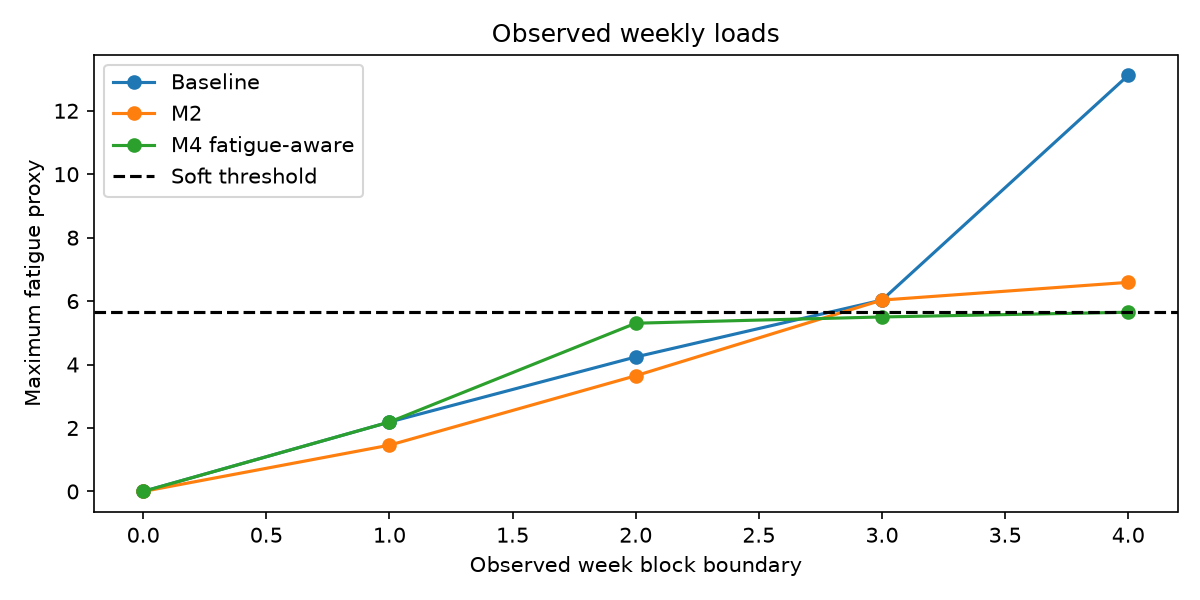
\includegraphics[width=0.78\textwidth]{figures/observed_fatigue.png}
\caption{Mức fatigue cực đại qua $4$ khối tuần lịch sử: M4 Fatigue-Aware giữ toàn bộ quỹ đạo dưới ngưỡng mềm $H = 5{,}660$ (tổng vượt ngưỡng $= 0{,}000$), giữ nguyên $\text{max\_load} = 11$ và $L_1 = 36{,}329$.}
\label{fig:m4_obs}
\end{figure}

\begin{figure}[htbp]
\centering
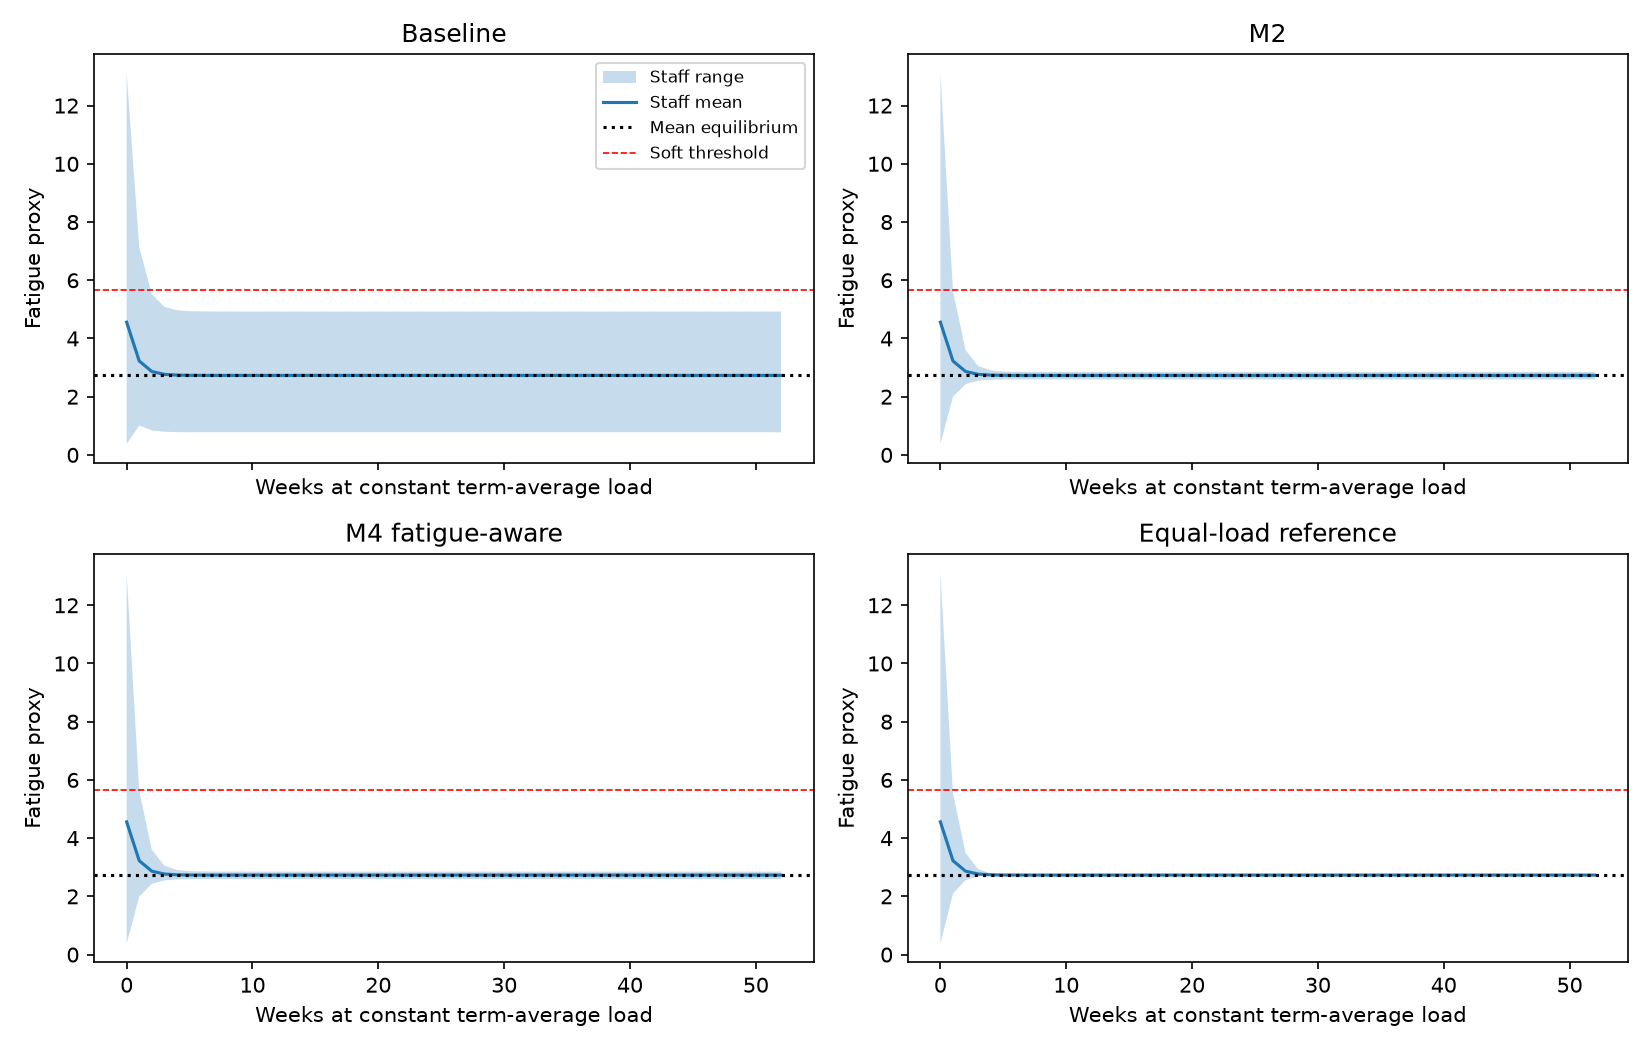
\includegraphics[width=0.86\textwidth]{figures/fatigue_equilibrium.png}
\caption{Quỹ đạo hội tụ $52$ tuần (dải $\min$--$\max$ và trung bình) dưới tải hằng kỳ đối với $4$ kịch bản, bắt đầu từ trạng thái cuối không đồng đều của Baseline.}
\label{fig:m4_eq}
\end{figure}

\begin{figure}[htbp]
\centering
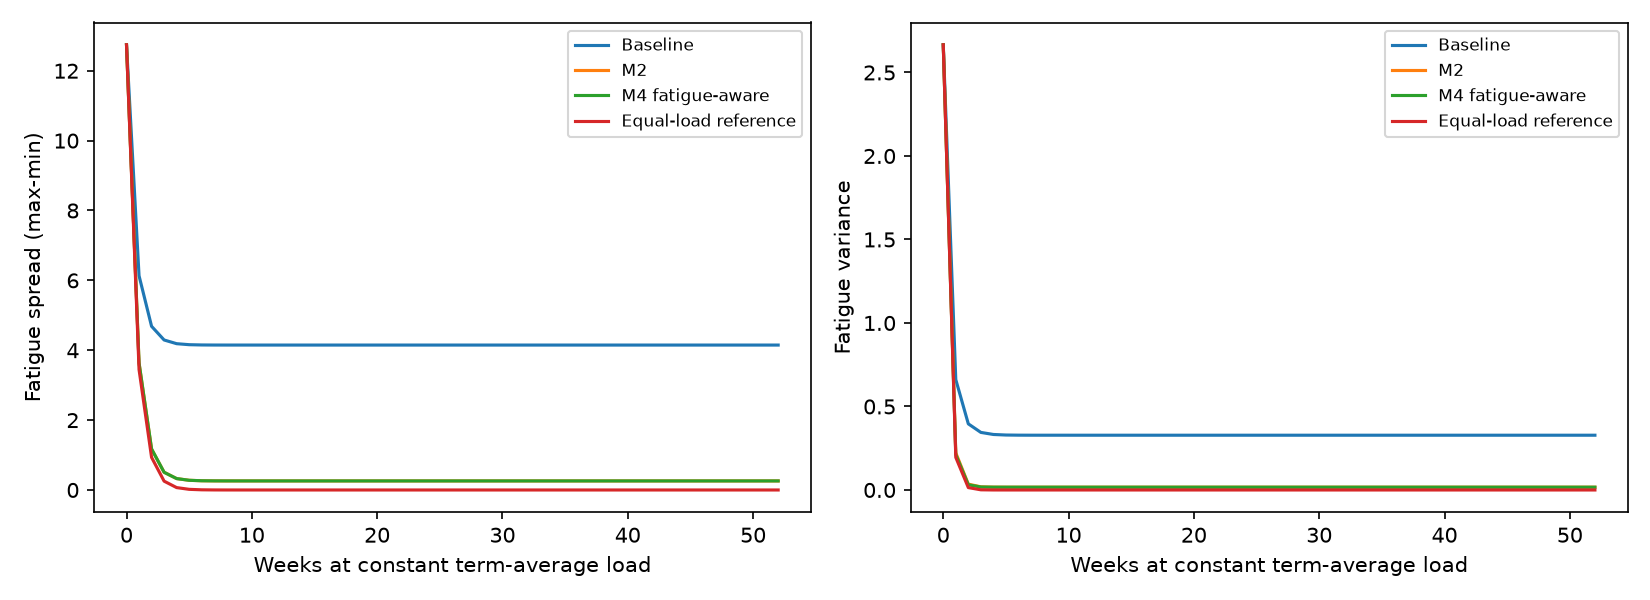
\includegraphics[width=0.86\textwidth]{figures/fairness.png}
\caption{Sự co hẹp theo hàm mũ của độ trải ($\operatorname{spread}$) và phương sai ($\operatorname{Var}$) fatigue theo thời gian, chứng minh tính chất hút công bằng của điểm cân bằng.}
\label{fig:m4_fair}
\end{figure}
\FloatBarrier